% =====================================================================
%  Workshop submission: KDD 2026 — Agentic Software Engineering Workshop
%  Format: 4-page position paper, ACM sigconf, anonymous, review
%  Version: v16 — overview figure and transaction-schema emphasis
%                  added after mentor review
%
%  Build:  latexmk -pdf token_tax.tex
% =====================================================================

\documentclass[sigconf,anonymous,review]{acmart}

\setcopyright{none}
\settopmatter{printacmref=false, printccs=false, printfolios=true}
\renewcommand\footnotetextcopyrightpermission[1]{}
\acmConference[KDD '26 Workshop]{KDD 2026 Workshop on
  Agentic Software Engineering}{August 10, 2026}{Jeju, Korea}

\usepackage{xcolor}
\usepackage{booktabs}
\usepackage{float}
\usepackage{xspace}
\usepackage{graphicx}
\usepackage{microtype}
\usepackage{tikz}
\usetikzlibrary{arrows.meta, positioning, fit, backgrounds}
\newcommand{\atm}{\textsc{Atm}\xspace}

\begin{document}

% =====================================================================
\title{Closing the AgentOps Loop:\\
       Runtime Transactions for AI Coding Agents}

\author{Anonymous Author(s)}
\affiliation{%
  \institution{Anonymous Institution}
  \country{}
}

% =====================================================================
\begin{abstract}
AI coding agents are becoming load-bearing parts of software
development, but Agentic SE still lacks a feedback loop for improving
how they behave in practice. Existing artifact datasets capture what
agents ultimately produce---patches, commits, pull requests, and
benchmark outcomes---but miss the runtime behavior that determines
cost, reliability, and productivity: retries, fallbacks, routing
decisions, failed repair loops, and abandoned sessions.

This position paper argues that the missing layer is not another
dashboard, but a closed-loop AgentOps substrate. We propose a five-stage
loop: \emph{agent execution} $\to$ \emph{runtime transactions} $\to$
\emph{behavioral analytics} $\to$ \emph{intervention} $\to$
\emph{measured improvement}. Such a loop would enable engineer coaching
grounded in behavioral evidence, workflow optimization at the stages
where agent tasks break down, and routing-policy iteration measured by
total task cost rather than per-request price.

We define the runtime transaction schema required to support this loop,
use \atm as a motivating local-first prototype, and identify three open
research problems: reconciling gateway and transcript traces without
shared request IDs, linking runtime sessions to asynchronous software
artifacts, and estimating whether interventions actually caused
improvement. We offer no population-level measurements; our contribution
is the architectural framing and research agenda for turning agent
observability into measurable improvement.
\end{abstract}

\keywords{AgentOps, feedback loops, runtime traces, AI coding agents,
  engineer coaching, routing policy, workflow optimization,
  local-first governance, agentic software engineering}

\maketitle

% =====================================================================
\section{Introduction}
\label{sec:intro}

Consider three scenarios that recur in agentic development practice.

\textbf{Vignette 1.} A developer's Claude Code session consumes
substantial cost and produces no commit. CI, git, and PR queues are
all empty. From every artifact-level signal, nothing happened. Yet
at runtime the agent issued multiple requests, hit a rate limit,
produced a malformed tool call, fell back to a cheaper model that
returned an incorrect patch, and terminated after several failed
repair attempts. The failure pattern is invisible to any dataset
built from artifacts~\cite{nakashima2026rejected, ehsani2026fail}.

\textbf{Vignette 2.} A team deploys a cost-aware routing policy:
coding tasks above 8K tokens route to a cheaper provider. The
per-request price drops 60\%. Two weeks later, total agent spend has
increased. No one knows why, because the gateway records only
resolved model and token count---not retry chains, fallback
frequency, or whether the task produced an accepted
patch~\cite{routecollapse2026, routingsurvey2026}.

\textbf{Vignette 3.} A senior and a junior engineer both use the
same coding agent on the same class of bug. The senior produces
accepted patches in two to three requests; the junior's sessions
average nine requests with three aborts. The difference is visible
in runtime traces---broad context selection, no plan step, repeated
retries without new information---but no system connects this
behavioral signal to a coaching recommendation~\cite{agentlens2026,
lu2025autonomous}.

Each vignette describes a situation where the information needed to
diagnose and fix the problem was present at runtime but was never
captured in a form that supports action. This is not a shortage of
algorithms: funnel analysis, cohort comparison, and policy A/B
testing are mature techniques. What is missing is the \emph{data
substrate}---the runtime transaction layer that would make these
techniques applicable to AI teammates. Without it, teams are left
choosing between ignoring the problem and guessing at the fix.

This paper makes three contributions. First, we argue that Agentic
SE needs a five-stage closed-loop AgentOps architecture connecting
runtime transactions to behavioral analytics, intervention, and
measured improvement (\S\ref{sec:loop}). Second, we define the
transaction schema that instantiates this loop---designed to
capture the five structural layers that artifact datasets lack---and
identify what current sources provide and what they lack
(\S\ref{sec:transactions}; see Figure~\ref{fig:overview} for the
full architecture). Third, we specify three concrete
feedback loops---engineer coaching, workflow optimization, and
routing policy iteration---with their required data, analytical
methods, interventions, and metrics (\S\ref{sec:loops}), use \atm
as a motivating prototype (\S\ref{sec:atm}), and pose three open
research problems whose solution is prerequisite to closing any of
the loops (\S\ref{sec:agenda}).

% =====================================================================
\section{Related Work}
\label{sec:related}

\paragraph{Artifact-centered Agentic SE.}
The dominant paradigm evaluates coding agents through what they
produce: resolve rate on SWE-bench~\cite{swebench2024, sweagent2024},
PR acceptance~\cite{nakashima2026rejected}, commit
quality~\cite{li2025se3}, and documentation~\cite{yamasaki2026docs}.
This approach is well suited to measuring agent capability on defined
tasks, but it systematically excludes the sessions that never produce
an artifact---failed, aborted, and retry-heavy executions that
generated cost without yielding a commit~\cite{ehsani2026fail,
mehtiyev2026beyond}. The exclusion is structural: artifact datasets
encode survivorship bias by construction~\cite{silentci2025,
abandonedprs2022}. Recent work has begun to acknowledge the blind
spot---AgentLens (arXiv:2605.12925) identifies ``lucky passes''
invisible to outcome-only evaluation~\cite{agentlens2026}; failure
trajectory analysis (arXiv:2511.00197) shows failed sessions are
consistently longer and higher-variance than successful
ones~\cite{majgaonkar2025trajectories}---but neither paper provides
infrastructure to act on these observations.

\paragraph{AgentOps and observability.}
Cloud platforms~\cite{langfuse, helicone, langsmith} and
OpenTelemetry instrumentation~\cite{openllmetry, otel-genai} provide
LLM tracing for applications where prompts can be forwarded to
centralized collectors---an assumption that fails for coding agents
whose payloads contain private source trees, credentials, and
unreleased features~\cite{infraagents2025}. Causal tracing systems
such as AgentTrace (arXiv:2602.10133)~\cite{agenttrace2026} localize
failure root causes in multi-agent systems, but presuppose a unified
trace already exists. We address the prior problem: collecting and
reconciling that trace locally from two independently maintained
sources without exfiltrating prompt content.

\paragraph{Behavioral analytics as a model.}
Product analytics practice demonstrates that observational data
becomes actionable only when connected to intervention and
re-measurement. Funnel analysis, cohort comparison, A/B experiments,
and metric trees are the standard toolkit for closing
observation-to-improvement loops in user-facing products. Agentic SE
has no equivalent: there is no established methodology for
identifying which agent behavior patterns lead to poor outcomes,
intervening on them, and measuring whether improvement followed.
Runtime transactions are the precondition for applying this toolkit
to AI teammates.

% =====================================================================
\section{The Missing Feedback Loop}
\label{sec:loop}

The artifact-only paradigm does not merely undersample the data it
needs---it structurally cannot collect it. Artifact datasets are
built from what agents leave behind: commits, pull requests, passing
tests, and benchmark solutions. Sessions that terminate without
producing an artifact leave nothing to scrape. The result is not
sampling error but the systematic exclusion of the sessions with the
most diagnostic value: failed repairs, abandoned tasks, and retry-heavy
executions that consumed substantial cost on the way to nothing.

We propose a five-stage architecture:

\begin{enumerate}
  \item \textbf{Agent execution.} Coding agents (Claude Code, Codex,
    Gemini CLI, OpenCode) run tasks on developer machines, generating
    gateway traffic and local transcript files.
  \item \textbf{Runtime transactions.} A local-first layer collects
    gateway logs and transcript logs independently, reconciles them
    into per-request records, and links them to session and task
    context.
  \item \textbf{Behavioral analytics.} Transaction records are
    aggregated into funnels, cohorts, policy comparisons, and cost
    attribution---the same primitives used in product analytics,
    applied to AI teammate behavior.
  \item \textbf{Intervention.} Diagnosis drives action: coaching
    recommendations, workflow template updates, routing policy
    changes, or guardrail adjustments.
  \item \textbf{Measured improvement.} Post-intervention transactions
    are compared against a baseline to verify the intervention worked.
\end{enumerate}

The loop fails if any stage is missing. A system that collects
transactions but provides no analytics is a log sink. A system that
diagnoses problems but tracks no outcomes is a dashboard. Only the
complete five-stage cycle constitutes a feedback loop---and each
stage places specific demands on the data that must be collected.

% =====================================================================
\section{Runtime Transactions}
\label{sec:transactions}

Figure~\ref{fig:overview} presents the architecture at a glance.
Token counts answer \emph{how much}. They do not answer \emph{why},
\emph{what happened}, or \emph{whether the routing decision was
correct}. A request consuming 10,000 input tokens might be a
successful refactor, a failed retry loop, or a policy-blocked
attempt that should never have reached that provider. The count is
identical in all three cases, which is precisely why token
accounting alone cannot support any of the three feedback loops.

\begin{figure*}[!t]
\centering
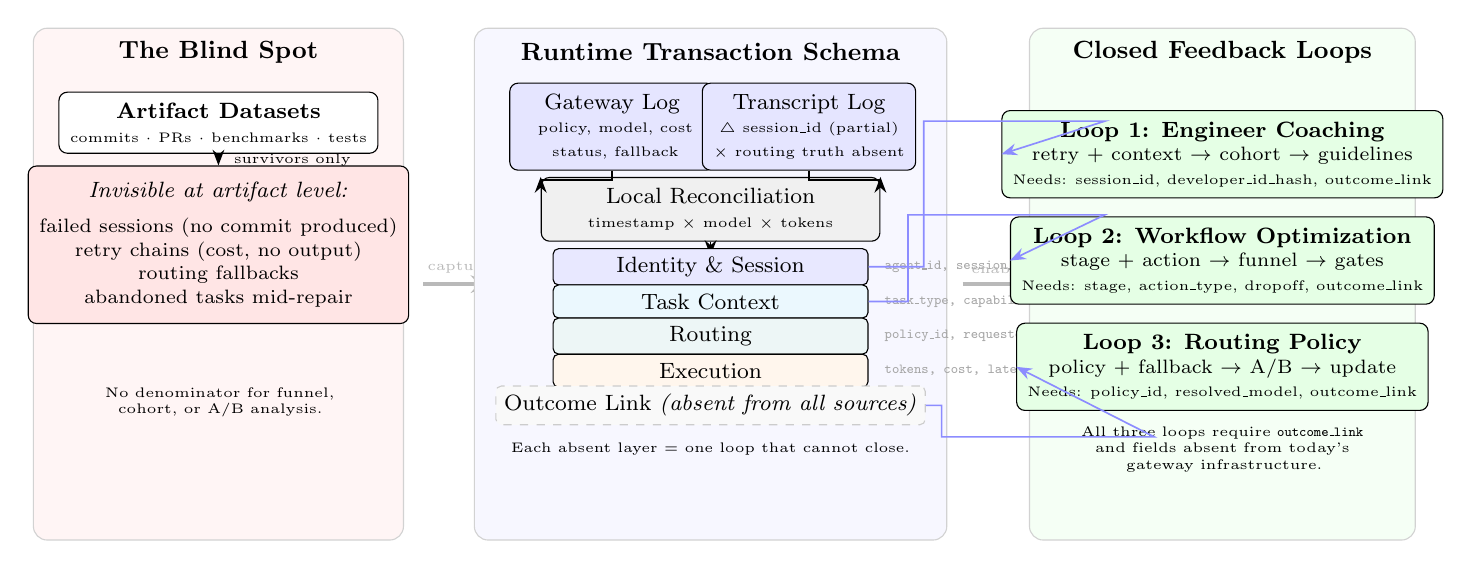
\begin{tikzpicture}[
  font=\footnotesize,
  arr/.style={-Stealth, semithick},
  panelbg/.style={draw=gray!35, rounded corners=5pt, inner sep=7pt},
  srcbox/.style={draw, rounded corners=3pt, align=center, inner sep=4pt,
                 minimum width=2.6cm, minimum height=0.65cm},
  layerbox/.style={draw, rounded corners=2pt, align=center, inner sep=3pt,
                   minimum width=4.0cm, minimum height=0.42cm},
  loopbox/.style={draw, rounded corners=3pt, align=center, inner sep=4pt,
                  minimum width=4.4cm, minimum height=0.72cm},
]

%% ─── PANEL 1: The Blind Spot ──────────────────────────────────────────────
\node[panelbg, fill=red!4, minimum width=4.7cm, minimum height=6.5cm]
  (p1bg) at (0,0) {};
\node[font=\small\bfseries] at (0, 2.95) {The Blind Spot};

\node[srcbox, fill=white, minimum width=3.9cm] at (0, 2.05) (artbox) {
  \textbf{Artifact Datasets}\\[-1pt]
  {\tiny commits~$\cdot$~PRs~$\cdot$~benchmarks~$\cdot$~tests}
};

\node[srcbox, fill=red!10, minimum width=3.9cm, minimum height=2.0cm]
  at (0, 0.5) (missbox) {
  \textit{Invisible at artifact level:}\\[3pt]
  {\scriptsize failed sessions (no commit produced)}\\[-1pt]
  {\scriptsize retry chains (cost, no output)}\\[-1pt]
  {\scriptsize routing fallbacks}\\[-1pt]
  {\scriptsize abandoned tasks mid-repair}
};

\draw[arr] (artbox.south) -- (missbox.north)
  node[midway, right=2pt, font=\tiny] {survivors only};

\node[font=\tiny, align=center, text width=3.8cm] at (0,-1.5) {
  No denominator for funnel,\\cohort, or A/B analysis.
};

%% ─── Arrow ────────────────────────────────────────────────────────────────
\draw[arr, very thick, color=gray!55] (2.6,0) -- ++(0.9,0)
  node[midway, above, font=\tiny] {capture};

%% ─── PANEL 2: Data Model ──────────────────────────────────────────────────
\node[panelbg, fill=blue!3, minimum width=6.0cm, minimum height=6.5cm]
  (p2bg) at (6.25,0) {};
\node[font=\small\bfseries] at (6.25, 2.95) {Runtime Transaction Schema};

\node[srcbox, fill=blue!10] at (5.0, 2.0) (gw) {
  Gateway Log\\[-1pt]{\tiny \checkmark~policy, model, cost}\\[-1pt]{\tiny \checkmark~status, fallback}
};
\node[srcbox, fill=blue!10] at (7.5, 2.0) (tr) {
  Transcript Log\\[-1pt]{\tiny $\triangle$~session\_id (partial)}\\[-1pt]{\tiny $\times$~routing truth absent}
};

\node[srcbox, fill=gray!12, minimum width=4.3cm] at (6.25, 0.95) (rec) {
  Local Reconciliation\\[-1pt]{\tiny timestamp $\times$ model $\times$ tokens}
};
\draw[arr] (gw.south) -- ++(0,-0.12) -| (rec.north west);
\draw[arr] (tr.south) -- ++(0,-0.12) -| (rec.north east);
\draw[arr] (rec.south) -- ++(0,-0.18);

\node[layerbox, fill=blue!9]   at (6.25,  0.22) (lid)  {Identity~\&~Session};
\node[layerbox, fill=cyan!8]   at (6.25, -0.22) (ltask){Task Context};
\node[layerbox, fill=teal!7]   at (6.25, -0.66) (lrout){Routing};
\node[layerbox, fill=orange!7] at (6.25, -1.10) (lexec){Execution};
\node[layerbox, fill=gray!5, draw=gray!40, dashed]
                               at (6.25, -1.54) (lout) {Outcome Link \emph{(absent from all sources)}};

\node[font=\tiny, color=gray!70, right=0.08cm of lid,  anchor=west]
  {\texttt{agent\_id,~session\_id,~developer\_id\_hash}};
\node[font=\tiny, color=gray!70, right=0.08cm of ltask, anchor=west]
  {\texttt{task\_type,~capability,~risk\_level}};
\node[font=\tiny, color=gray!70, right=0.08cm of lrout, anchor=west]
  {\texttt{policy\_id,~requested\_model,~resolved\_model}};
\node[font=\tiny, color=gray!70, right=0.08cm of lexec, anchor=west]
  {\texttt{tokens,~cost,~latency,~status,~retry\_count}};

\node[font=\tiny, align=center] at (6.25,-2.1)
  {Each absent layer $=$ one loop that cannot close.};

%% ─── Arrow ────────────────────────────────────────────────────────────────
\draw[arr, very thick, color=gray!55] (9.45,0) -- ++(0.9,0)
  node[midway, above, font=\tiny] {enable};

%% ─── PANEL 3: Feedback Loops ──────────────────────────────────────────────
\node[panelbg, fill=green!4, minimum width=4.9cm, minimum height=6.5cm]
  (p3bg) at (12.75,0) {};
\node[font=\small\bfseries] at (12.75, 2.95) {Closed Feedback Loops};

\node[loopbox, fill=green!10] at (12.75,  1.65) (lp1) {
  \textbf{Loop 1: Engineer Coaching}\\[-1pt]
  {\scriptsize retry + context $\to$ cohort $\to$ guidelines}\\[-1pt]
  {\tiny Needs: session\_id, developer\_id\_hash, outcome\_link}
};
\node[loopbox, fill=green!10] at (12.75,  0.3) (lp2) {
  \textbf{Loop 2: Workflow Optimization}\\[-1pt]
  {\scriptsize stage + action $\to$ funnel $\to$ gates}\\[-1pt]
  {\tiny Needs: stage, action\_type, dropoff, outcome\_link}
};
\node[loopbox, fill=green!10] at (12.75, -1.05) (lp3) {
  \textbf{Loop 3: Routing Policy}\\[-1pt]
  {\scriptsize policy + fallback $\to$ A/B $\to$ update}\\[-1pt]
  {\tiny Needs: policy\_id, resolved\_model, outcome\_link}
};

\node[font=\tiny, align=center, text width=4.3cm] at (12.75,-2.1) {
  All three loops require \texttt{outcome\_link}\\
  and fields absent from today's\\gateway infrastructure.
};

%% ─── Connections schema → loops ──────────────────────────────────────────
\draw[arr, color=blue!45]
  (lout.east)  -- ++(0.2,0) -- ++(0,-0.4) -- ++(2.7,0) -- (lp3.west);
\draw[arr, color=blue!45]
  (ltask.east) -- ++(0.5,0) -- ++(0, 1.1) -- ++(2.5,0) -- (lp2.west);
\draw[arr, color=blue!45]
  (lid.east)   -- ++(0.7,0) -- ++(0, 1.85)-- ++(2.3,0) -- (lp1.west);

\end{tikzpicture}
\caption{The AgentOps feedback architecture in three panels.
  \emph{Left}: artifact-only datasets structurally exclude every session that
  does not produce a commit, eliminating the denominator required for
  behavioral analysis.
  \emph{Center}: the runtime transaction schema fills this gap by assembling
  five logical layers from two locally-maintained sources; each absent layer
  directly blocks the feedback loop that depends on it.
  \emph{Right}: the three closed feedback loops each require schema fields
  that no existing coding-agent data source provides; all three share a
  common prerequisite in \texttt{outcome\_link}.}
\label{fig:overview}
\end{figure*}

The data model is designed around a single insight: the observability
problem is not one of instrumentation volume but of \emph{structural
absence}. Artifact datasets cannot be patched into a feedback
substrate---they capture only the tail of a session, not its runtime
body. The model therefore starts from the runtime request and builds
upward, adding context layers that artifact records structurally
lack.

What each loop requires is a runtime transaction: a record
that captures five dimensions simultaneously. \textbf{Identity}
establishes which agent, which developer session, and which source
tool initiated the request---the anchor for engineer-level cohort
analysis. Without \texttt{developer\_id\_hash} and
\texttt{session\_id}, failed sessions cannot be attributed to any
engineer, and the coaching loop has no subject.
\textbf{Task context} situates the request within a task type,
capability, risk level, and project. Without \texttt{task\_type},
routing policies cannot be evaluated per capability, and the routing
loop conflates bugfix requests with documentation requests even when
their optimal model assignments differ.
\textbf{Routing} records the policy applied, the model the agent
requested, and the provider and model that actually served the
request---the fields that make substitution detectable and policy
evaluation possible. Gateway logs provide these; transcript logs do
not.
\textbf{Execution} records tokens, cost, latency,
status, failure type, fallback reason, and retry count, supporting
failure taxonomy and retry analysis. Both sources provide partial
coverage here; reconciliation is required to populate all fields.
\textbf{Outcome} optionally links the request to a downstream test
result, PR, or human acceptance decision---the join key that closes
the loop between execution and improvement.
This layer is currently absent from every coding-agent data source,
and its absence is the single most consequential gap in the
infrastructure: without it, no loop can compute its primary metric.

Table~\ref{tab:schema} shows the minimal schema spanning these
dimensions. Fully supporting all three loops requires five logical
objects: \texttt{AgentSession}, \texttt{AgentTask},
\texttt{AgentAction}, \texttt{RuntimeTransaction}, and
\texttt{OutcomeLink}. Gateway-only systems provide the transaction
row but lack session, task, and outcome context. Transcript-only
systems provide session context but lack routing truth. Neither
source alone can populate the full schema; both are necessary, and
their reconciliation is where the analytical value is created.

\begin{table}[t]
\caption{Minimal runtime transaction schema. Each layer contributes
  fields that a different feedback loop depends on.}
\label{tab:schema}
\small
\begin{tabular}{@{}p{1.2cm}p{3.2cm}p{2.25cm}@{}}
\toprule
\textbf{Layer} & \textbf{Field} & \textbf{Enables} \\
\midrule
Identity   & \texttt{agent\_id}, \texttt{developer\_id\_hash}       & Engineer cohorts \\
           & \texttt{session\_id}, \texttt{source\_tool}            & Session funnels \\
Task       & \texttt{task\_type}, \texttt{capability}               & Capability routing \\
           & \texttt{risk\_level}, \texttt{project\_id}             & Audit, attribution \\
Routing    & \texttt{policy\_id}, \texttt{requested\_model}         & Policy cohorts \\
           & \texttt{provider}, \texttt{resolved\_model}            & Substitution detect \\
Execution  & \texttt{tokens}, \texttt{cost\_usd}, \texttt{latency\_ms} & Cost attribution \\
           & \texttt{status}, \texttt{failure\_type}                & Failure taxonomy \\
           & \texttt{fallback\_reason}, \texttt{retry\_count}       & Retry analysis \\
Outcome    & \texttt{outcome\_link}                                 & Loop closure \\
\bottomrule
\end{tabular}
\end{table}

% =====================================================================
\section{Three Feedback Loops}
\label{sec:loops}

With the schema in place, we can specify what each feedback loop
requires---not just in terms of data fields, but as a connected
sequence from blind spot to measured improvement. Table~\ref{tab:loops}
summarizes all three; the subsections develop each argument in full.

\begin{table}[t]
\caption{Three closed AgentOps feedback loops. Each requires distinct
  data signals unavailable from artifact datasets alone.}
\label{tab:loops}
\small
\begin{tabular}{@{}p{1.05cm}p{1.6cm}p{1.35cm}p{1.15cm}p{1.1cm}@{}}
\toprule
\textbf{Loop} & \textbf{Signal} & \textbf{Method} & \textbf{Action} & \textbf{Metric} \\
\midrule
Engineer coaching
  & retry\_count, context size, abort, outcome
  & Cohort + before/after
  & Workflow coaching
  & Cost/accepted patch $\downarrow$ \\
\midrule
Workflow optim.
  & stage, dropoff, failure type, action sequence
  & Funnel + sequence mining
  & Test gates, context packs
  & Completion rate $\uparrow$ \\
\midrule
Routing iteration
  & policy, capability, resolved model, fallback, outcome
  & Policy cohort, A/B
  & Policy update
  & Total cost/task $\downarrow$ \\
\bottomrule
\end{tabular}
\end{table}

\subsection{Loop 1: Engineer Coaching}

Artifact datasets record who submitted a PR, not who retried nine
times before aborting. Two engineers producing equal numbers of
accepted patches are indistinguishable in any commit-level dataset,
even when one consistently consumes five times the tokens getting
there~\cite{agentlens2026, mehtiyev2026beyond}. Runtime traces break
this symmetry: they expose behavioral fingerprints that separate
efficient usage from wasteful usage---broad context selection, absent
plan steps, retries that add no new information to the context,
high abort rates on task types where other engineers succeed.

These signals make cohort analysis possible. By grouping engineers
according to observed usage patterns---broad-context versus scoped,
plan-first versus direct-edit---and comparing cost per accepted
patch and abandoned session rate across groups, it becomes possible
to identify which patterns systematically correlate with poor
outcomes. When a ``high retry + broad context'' cohort shows
consistently higher cost and lower completion, the diagnosis is
specific enough to drive a targeted intervention: coaching on
plan-first and scoped-context workflows, updated team usage
guidelines, or task decomposition templates for the task types
where the pattern concentrates. Improvement is confirmed when
post-coaching traces for the coached cohort show lower retry tokens
per accepted patch and lower abandoned session rate---a before-after
comparison that artifact datasets cannot support because they do not
record the behavioral signal in the first place.

This loop currently cannot be instantiated because
\texttt{developer\_id\_hash}, \texttt{session\_id},
\texttt{task\_type}, and \texttt{outcome\_link} are absent from
all existing coding-agent gateway systems. Treating these fields
as first-class infrastructure requirements, rather than optional
telemetry, is the minimum change needed to make engineer coaching
evidence-based rather than intuitive.

\subsection{Loop 2: Workflow Optimization}

Where Loop~1 operates at the level of individual engineer behavior,
Loop~2 operates at the level of task structure---asking not how a
particular developer uses the agent, but where in the multi-stage
workflow agent-assisted tasks most commonly break down.

Request-level logs are a call list without a call stack: they record
that something failed, not where in the context-gathering, planning,
editing, testing, and repair sequence the breakdown occurred~\cite{%
majgaonkar2025trajectories, lu2025autonomous}. Prior work on failure
trajectories (arXiv:2511.00197) establishes that failed sessions
are longer and higher-variance than successful ones, but it cannot
pinpoint which stage to fix without stage-level instrumentation.
Once stage boundaries and action sequences are recorded, funnel
analysis computes per-stage conversion rates from task started to
artifact accepted, sequence mining identifies recurring failure
paths such as ``edit $\to$ skip test $\to$ repair $\to$ abort,''
and survival analysis locates the stage at which tasks are most
likely to be abandoned permanently.

The diagnosis is then specific enough to drive stage-targeted
interventions: scoped context packs for sessions that stall at
context gathering, forced test gates for sessions that skip from
edit directly to repair, repair-loop limits for sessions that
retry without convergence. Completion rate and time to accepted
commit measure whether the intervention worked. This loop requires
\texttt{stage}, \texttt{action\_type}, \texttt{dropoff\_stage},
and \texttt{outcome\_link}---fields that no current coding-agent
gateway records. Extending from request-level to workflow-level
modeling is the single most consequential infrastructure gap
for this loop.

\subsection{Loop 3: Routing Policy Iteration}

Routing policies are today configured by intuition and evaluated,
if at all, on benchmark quality metrics that bear little relation to
real-agent retry and fallback behavior~\cite{routingsurvey2026}.
The specific failure mode that motivates this loop---a cheaper
routing policy that reduces per-request cost while increasing retry
frequency and total task cost---appears in no existing empirical
study; routing surveys (arXiv:2603.04445) explicitly identify it as
an open measurement gap~\cite{routingsurvey2026, routecollapse2026}.
The gap exists precisely because measuring total task cost requires
\texttt{outcome\_link}: without knowing whether a task produced an
accepted artifact, there is no denominator for the cost-per-completed-task
metric that distinguishes a cheap-per-request policy from a
cheap-per-outcome policy.

With outcome linkage in place, policy cohort analysis can compare
total cost per completed task, fallback rate, and success rate across
policy groups for the same capability and task type. A/B assignment
provides controlled comparison; bandit-style learning can update
routing weights dynamically based on observed outcomes~\cite{%
frugalgpt2023, routellm2024}. The intervention follows directly from
the diagnosis: reroute bugfix tasks from cheap-first to
reliable-first when fallback rate exceeds a threshold, lock
documentation tasks to cheaper models when quality differences are
undetectable, remove providers that consistently time out on
long-context capability. Among the three loops, this one is closest
to achievable with current infrastructure---most routing fields are
already recorded---making it the natural starting point for any
team that wants to begin closing the AgentOps loop today.

% =====================================================================
\section{\atm as a Motivating Prototype}
\label{sec:atm}

\atm\footnote{Anonymized for review; open-source link in
camera-ready.} is a local-first desktop application that
instantiates the transaction substrate described in
\S\ref{sec:transactions} by assembling two independently
maintained evidence sources on the developer's machine, without
forwarding any prompt content to external collectors.
Figure~\ref{fig:atm} shows the coverage each source provides
and the gap that remains.

\begin{figure}[t]
\centering
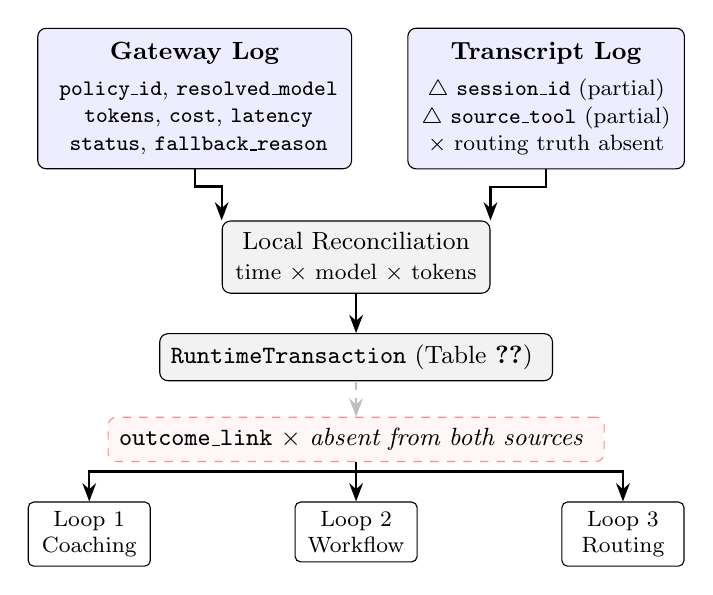
\begin{tikzpicture}[
  font=\small,
  srcbox/.style={draw, rounded corners=3pt, align=center, inner sep=5pt,
                 minimum width=3.4cm, minimum height=1.0cm},
  pipe/.style={draw, rounded corners=3pt, align=center, inner sep=4pt,
               minimum width=3.4cm, minimum height=0.55cm, fill=gray!10},
  missingbox/.style={draw=red!45, dashed, rounded corners=3pt, align=center,
                     inner sep=4pt, minimum width=3.4cm,
                     minimum height=0.55cm, fill=red!3},
  arr/.style={-Stealth, thick},
  dasharr/.style={-Stealth, thick, dashed, draw=gray!50},
]

% Two sources
\node[srcbox, fill=blue!7] (gw) {
  \textbf{Gateway Log}\\[2pt]
  {\footnotesize \checkmark~\texttt{policy\_id}, \texttt{resolved\_model}}\\[-1pt]
  {\footnotesize \checkmark~\texttt{tokens}, \texttt{cost}, \texttt{latency}}\\[-1pt]
  {\footnotesize \checkmark~\texttt{status}, \texttt{fallback\_reason}}
};

\node[srcbox, fill=blue!7, right=0.7cm of gw] (tr) {
  \textbf{Transcript Log}\\[2pt]
  {\footnotesize $\triangle$~\texttt{session\_id}~(partial)}\\[-1pt]
  {\footnotesize $\triangle$~\texttt{source\_tool}~(partial)}\\[-1pt]
  {\footnotesize $\times$~routing truth absent}
};

% Reconciliation
\node[pipe, below=0.65cm of gw, xshift=2.05cm] (rec) {
  Local Reconciliation\\{\footnotesize time $\times$ model $\times$ tokens}
};
\draw[arr] (gw.south)  -- ++(0,-0.22) -| (rec.north west);
\draw[arr] (tr.south)  -- ++(0,-0.22) -| (rec.north east);

% RuntimeTransaction
\node[pipe, below=0.5cm of rec] (txn) {
  \texttt{RuntimeTransaction}~(Table~\ref{tab:schema})
};
\draw[arr] (rec) -- (txn);

% Missing outcome link
\node[missingbox, below=0.45cm of txn] (out) {
  \texttt{outcome\_link}~$\times$~\emph{absent from both sources}
};
\draw[dasharr] (txn) -- (out);

% Loops at bottom
\node[draw, rounded corners=2pt, align=center, font=\footnotesize,
      minimum width=1.55cm, below left=0.5cm and -0.55cm of out] (l1)
  {Loop~1\\Coaching};
\node[draw, rounded corners=2pt, align=center, font=\footnotesize,
      minimum width=1.55cm, below=0.5cm of out] (l2)
  {Loop~2\\Workflow};
\node[draw, rounded corners=2pt, align=center, font=\footnotesize,
      minimum width=1.55cm, below right=0.5cm and -0.55cm of out] (l3)
  {Loop~3\\Routing};

\draw[arr] (out.south) -- ++(0,-0.12) -| (l1.north);
\draw[arr] (out.south) -- (l2.north);
\draw[arr] (out.south) -- ++(0,-0.12) -| (l3.north);

\end{tikzpicture}
\caption{\atm dual-source reconciliation. Gateway logs provide routing
  truth (\checkmark); transcript logs provide partial session context
  ($\triangle$); each source lacks what the other records, making
  reconciliation the value-creating step. \texttt{outcome\_link}
  ($\times$) is absent from both sources and is the minimum addition
  needed to compute total-task cost for any of the three loops.}
\label{fig:atm}
\end{figure}

When an agent uses an \atm-issued per-agent key, requests pass
through a local HTTP gateway that records agent identity, policy,
resolved provider and model, token counts, latency, status, and
fallback behavior---without storing any prompt content. In parallel,
\atm scans on-disk history files from Claude Code, Codex, Gemini
CLI, and other tools, aggregating them into daily rollups keyed by
application, model label, and time window. The two pipelines
populate separate tables; reconciliation happens only after both
sources have been written locally, preserving the independence of
each evidence source.

This architecture already supports Loop~3: routing fields
(\texttt{policy\_id}, \texttt{resolved\_model}, \texttt{tokens},
\texttt{cost}, \texttt{latency}, \texttt{status},
\texttt{fallback\_reason}) are fully recorded, and the reconciled
table directly expresses the two diagnostic states that motivate
the loop---subscription bypass (gateway absent, transcript present)
and model-label divergence (requested model $\neq$ resolved model).
What is absent is \texttt{outcome\_link}, the single field that
separates per-request cost accounting from total-task cost
attribution. Loops~1 and~2 require additional fields not yet
collected: \texttt{session\_id}, \texttt{developer\_id\_hash},
\texttt{task\_type}, \texttt{stage}, and \texttt{action\_type}.
Our position is that Agentic SE should treat these as first-class
infrastructure requirements, not optional telemetry, because no
feedback loop can be closed without them.

% =====================================================================
\section{Open Research Problems}
\label{sec:agenda}

Three research problems must be solved before the loops above can
be closed at scale; each is harder in the agentic setting than its
surface resemblance to prior work suggests.

\textbf{Trace reconciliation without shared request IDs.}
Probabilistic record linkage---matching gateway log entries to
transcript entries on timestamp, model name, and token count---is
theoretically grounded~\cite{fellegi1969theory, splink2022}, but
the agentic setting introduces a challenge that classical entity
resolution does not face: some transcript entries have no
corresponding gateway record not because the join failed, but
because the agent ran in subscription mode and the gateway never
saw the request. Absence is not missing data---it is a diagnostic
state. Standard record-linkage models that assume both sources
describe the same population must be redesigned for a setting where
one-sided observations carry their own semantic meaning, and where
distinguishing a failed join from a genuine subscription-bypass
event is itself an open algorithmic problem. Solving this is
prerequisite to Loops~1 and~3, both of which depend on correctly
attributing agent activity across authentication modes.

\textbf{Outcome linking across asynchronous systems.}
An agent session may produce a commit hours after the requests
complete, or may produce no artifact at all. Linking runtime
transactions to downstream test results, PR reviews, and human
acceptance decisions without a shared key across all systems is an
open record-linkage problem~\cite{linktransformer2024}. The harder
case is the no-artifact session: it must be classified as a failure,
but the absence of an artifact is indistinguishable from a session
whose artifact has not yet been produced---a temporal ambiguity that
requires either timeout heuristics or explicit agent-side signaling.
Without reliable outcome linking, none of the three loops can
compute total task cost, completion rate, or cost per accepted
patch, which are the metrics that distinguish policy improvement
from noise.

\textbf{Intervention causality.}
Confirming that a coaching session or policy update \emph{caused}
improvement is confounded by task-mix shifts, model version updates,
and natural developer learning curves. Causal inference designs
suitable for Agentic SE---difference-in-differences, synthetic
control, regression discontinuity---have not been studied in this
setting, where the unit of treatment is a developer or a routing
policy, not a randomized user~\cite{trail2025}. Without valid
causal designs, the measured improvement stage of the loop cannot
be trusted, and teams have no way to distinguish a genuine
intervention effect from a favorable shift in workload composition.

% =====================================================================
\section{Conclusion}
\label{sec:conclusion}


Agentic SE has largely evaluated AI coding agents by their outputs:
patches, commits, pull requests, and benchmark results. This view is
necessary, but it is not sufficient for improving agentic development
in practice. Many of the behaviors that determine cost, reliability,
and productivity occur before an artifact exists: retries, fallbacks,
routing decisions, abandoned sessions, and repair loops.

We argued that Agentic SE needs a closed-loop AgentOps substrate that
turns these runtime behaviors into transaction records, turns
transactions into behavioral analytics, and turns analytics into
interventions whose effects can be measured. The central challenge is
not simply to log more events, but to collect the right metadata,
reconcile partial traces, link execution to outcomes, and evaluate
whether changes to training, workflows, or routing policies actually
improve development.

The broader position is that AI teammates should be treated as
improvable participants in the software process, not only as systems
to benchmark after the fact. Closing the AgentOps loop would make it
possible to coach engineers with behavioral evidence, redesign
agent-assisted workflows around observed failure points, and iterate
routing policies against real task outcomes. Building this loop is the
infrastructure work required for accountable, measurable, and
continuously improving agentic software engineering.

% =====================================================================
\bibliographystyle{ACM-Reference-Format}
\bibliography{refs}

\end{document}
